\ifx\wholebook\relax \else
% ------------------------ 

\documentclass{article}
%------------------- Other types of document example ------------------------
%
%\documentclass[twocolumn]{IEEEtran-new}
%\documentclass[12pt,twoside,draft]{IEEEtran}
%\documentstyle[9pt,twocolumn,technote,twoside]{IEEEtran}
%
%-----------------------------------------------------------------------------
%%
% loading packages
%
\newif\ifpdf
\ifx\pdfoutput\undefined % We're not running pdftex
  \pdffalse
\else
  \pdftrue
\fi
%
%
\ifpdf
  \RequirePackage[pdftex,%
            CJKbookmarks,%
       bookmarksnumbered,%
              colorlinks,%
          linkcolor=blue,%
              hyperindex,%
        plainpages=false,%
       pdfstartview=FitH]{hyperref}
\else
  \RequirePackage[dvipdfm,%
             CJKbookmarks,%
        bookmarksnumbered,%
               colorlinks,%
           linkcolor=blue,%
               hyperindex,%
         plainpages=false,%
        pdfstartview=FitH]{hyperref}
  \AtBeginDvi{\special{pdf:tounicode GBK-EUC-UCS2}} % GBK -> Unicode
\fi
\usepackage{hyperref}

% other packages
%-----------------------------------------------------------------------------
\usepackage{graphicx, color}
\usepackage{CJK}
%
% for programming 
%
\usepackage{verbatim}
\usepackage{listings}


\lstdefinelanguage{Smalltalk}{
  morekeywords={self,super,true,false,nil,thisContext}, % This is overkill
  morestring=[d]',
  morecomment=[s]{"}{"},
  alsoletter={\#:},
  escapechar={!},
  literate=
    {BANG}{!}1
    {UNDERSCORE}{\_}1
    {\\st}{Smalltalk}9 % convenience -- in case \st occurs in code
    % {'}{{\textquotesingle}}1 % replaced by upquote=true in \lstset
    {_}{{$\leftarrow$}}1
    {>>>}{{\sep}}1
    {^}{{$\uparrow$}}1
    {~}{{$\sim$}}1
    {-}{{\sf -\hspace{-0.13em}-}}1  % the goal is to make - the same width as +
    %{+}{\raisebox{0.08ex}{+}}1		% and to raise + off the baseline to match -
    {-->}{{\quad$\longrightarrow$\quad}}3
	, % Don't forget the comma at the end!
  tabsize=2
}[keywords,comments,strings]

\lstloadlanguages{C++, Lisp, Haskell, Python, Smalltalk}

% ======================================================================

\def\BibTeX{{\rm B\kern-.05em{\sc i\kern-.025em b}\kern-.08em
    T\kern-.1667em\lower.7ex\hbox{E}\kern-.125emX}}

\newtheorem{theorem}{Theorem}

%
% mathematics
%
\newcommand{\be}{\begin{equation}}
\newcommand{\ee}{\end{equation}}
\newcommand{\bmat}[1]{\left( \begin{array}{#1} }
\newcommand{\emat}{\end{array} \right) }
\newcommand{\VEC}[1]{\mbox{\boldmath $#1$}}

% numbered equation array
\newcommand{\bea}{\begin{eqnarray}}
\newcommand{\eea}{\end{eqnarray}}

% equation array not numbered
\newcommand{\bean}{\begin{eqnarray*}}
\newcommand{\eean}{\end{eqnarray*}}

\RequirePackage{CJK,CJKnumb,CJKulem,CJKpunct}
% we use CJK as default environment
\AtBeginDocument{\begin{CJK*}{GBK}{song}\CJKtilde\CJKindent\CJKcaption{GB}}
\AtEndDocument{\clearpage\end{CJK*}}

%
% loading packages
%

\RequirePackage{ifpdf}

%
%
\ifpdf
  \RequirePackage[pdftex,%
       bookmarksnumbered,%
              colorlinks,%
          linkcolor=blue,%
              hyperindex,%
        plainpages=false,%
       pdfstartview=FitH]{hyperref}
\else
  \RequirePackage[dvipdfm,%
        bookmarksnumbered,%
               colorlinks,%
           linkcolor=blue,%
               hyperindex,%
         plainpages=false,%
        pdfstartview=FitH]{hyperref}
\fi
\usepackage{hyperref}

% other packages
%--------------------------------------------------------------------------
\usepackage{graphicx, color}
\usepackage{subfig}

\usepackage{amsmath, amsthm, amssymb} % for math
\usepackage{exercise} % for exercise

%
% for programming 
%
\usepackage{verbatim}
\usepackage{listings}
%\usepackage{algorithmic} %old version; we can use algorithmicx instead
\usepackage{algorithm} 
\usepackage[noend]{algpseudocode} %for pseudo code, include algorithmicsx automatically
\usepackage{makeidx} % for index support


\lstdefinelanguage{Smalltalk}{
  morekeywords={self,super,true,false,nil,thisContext}, % This is overkill
  morestring=[d]',
  morecomment=[s]{"}{"},
  alsoletter={\#:},
  escapechar={!},
  literate=
    {BANG}{!}1
    {UNDERSCORE}{\_}1
    {\\st}{Smalltalk}9 % convenience -- in case \st occurs in code
    % {'}{{\textquotesingle}}1 % replaced by upquote=true in \lstset
    {_}{{$\leftarrow$}}1
    {>>>}{{\sep}}1
    {^}{{$\uparrow$}}1
    {~}{{$\sim$}}1
    {-}{{\sf -\hspace{-0.13em}-}}1  % the goal is to make - the same width as +
    %{+}{\raisebox{0.08ex}{+}}1		% and to raise + off the baseline to match -
    {-->}{{\quad$\longrightarrow$\quad}}3
	, % Don't forget the comma at the end!
  tabsize=2
}[keywords,comments,strings]

\lstloadlanguages{C++, Lisp, Haskell, Python, Smalltalk}

% ======================================================================

\def\BibTeX{{\rm B\kern-.05em{\sc i\kern-.025em b}\kern-.08em
    T\kern-.1667em\lower.7ex\hbox{E}\kern-.125emX}}

%
% mathematics
%
\newcommand{\be}{\begin{equation}}
\newcommand{\ee}{\end{equation}}
\newcommand{\bmat}[1]{\left( \begin{array}{#1} }
\newcommand{\emat}{\end{array} \right) }
\newcommand{\VEC}[1]{\mbox{\boldmath $#1$}}

% numbered equation array
\newcommand{\bea}{\begin{eqnarray}}
\newcommand{\eea}{\end{eqnarray}}

% equation array not numbered
\newcommand{\bean}{\begin{eqnarray*}}
\newcommand{\eean}{\end{eqnarray*}}

\newtheorem{theorem}{Theorem}[section]
\newtheorem{lemma}[theorem]{Lemma}
\newtheorem{proposition}[theorem]{Proposition}
\newtheorem{corollary}[theorem]{Corollary}


\setcounter{page}{1}

\begin{document}

\fi
%--------------------------

% ================================================================
%                 COVER PAGE
% ================================================================

\title{Trie, Patricia, and Suffix tree, with Functional and imperative implementation}

\author{Liu~Xinyu
\thanks{{\bfseries Liu Xinyu } \newline
  Email: liuxinyu95@gmail.com \newline}
%  Tel:   +86-1305-196-8666 \newline}
  }

\markboth{Trie, Patricia, and Suffix tree}
{imperative and functional implementation}

\maketitle

\ifx\wholebook\relax
\chapter{Trie, Patricia, and Suffix tree, with Functional and imperative implementation}

\section{abstract}
\else
\begin{abstract}
\fi
Trie, Patricia, and Suffix tree are important data structures in
information retreiving and manipulating. None of these data structures
are new. They were invented in 1960s. This post collects some
existing knowledge about them. Some functional and imperative
implementation are given in order to show the basic idea of these data structures.
There are multiple programming languages used, including, C++, Haskell, python and scheme/lisp.
C++ and python are mostly used to show the imperative implementation, while Haskell and Scheme are
used for functional purpose.

There may be mistakes in the post, please feel free to point out.

This post is generated by \LaTeXe, and provided with GNU FDL(GNU Free Documentation License).
Please refer to http://www.gnu.org/copyleft/fdl.html for detail.

\ifx\wholebook\relax\else
\end{abstract}
\fi

\vspace{3cm}
{\bfseries Keywords:} Trie, Patricia, Radix tree, Suffix tree

%{\bfseries Corresponding Author:} Liu Xinyu

\maketitle

% ================================================================
%                 Introduction
% ================================================================
\section{Introduction}
\label{introduction}

There isn't a seperate chapter about Trie, Patricia, ans Suffix tree
in CLRS book. While these data structure are very basic, especially in
information retrieving. Some of them are also widely used in
compiler design\cite{okasaki-int-map}, and bio-information area, such as
DNA pattern matching \cite{wiki-suffix-tree}.

In CLRS book index, Trie is redirected to Radix tree, while Radix tree
is described in Problem 12-1 \cite{CLRS}.

\begin{figure}[htbp]
       \begin{center}
	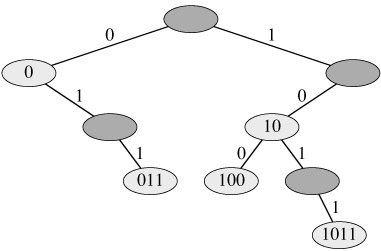
\includegraphics[scale=0.5]{img/radix-tree.eps}
        \caption{an Radix tree example in CLRS} \label{fig:radix-tree}
       \end{center}
\end{figure}

Figure \ref{fig:radix-tree} shows a radix tree contains the bit
strings 1011, 10, 011, 100 and 0. When searching for a key $k=b_0b_1...b_n$, we
take the first bit $b_0$ (MSB from left), check if it is 0 or 1, if it
is 0, we turn left, and turn right for 1. Then we take the 2nd bit and
repeat this search until we either meet a leaf or finish all n bits.

Note that radix tree needn't store any key in node at all. The
infomation are represented by edges in fact. The node with key string
in the above figure are only for illustration.

It is very natural to come to the idea `is it possible to represent
keys in integers instead of string, because integer can be denoted in
binary format?'. Such approach can save spaces and it is fast if we
can use bitwise manipulation.

I'll first show the integer Trie data structure and implementation in
section \ref{int-trie}. Then we can point out the drawbacks and go to
the improved data structure of integer Patricia in
section \ref{int-patricia}.
After that, I'll show alphabetic Trie and Patricia and list some
typicall use of them in textual manipulation engineering problems.
I'll show Suffix tree data structure and linear time contruction
algorithm in section \ref{suffix-tree}.

This article provides example implementation of Trie, Patricia and Suffix tree
in C, C++, Haskell, Python, and Scheme/Lisp languages. Some functional
implementation can be referenced from current Haskell packages \ref{hackage-int-map} 
\ref{hackage-bytestring-map}.

All source code can be downloaded in appendix \ref{appendix}, please 
refer to appendix for detailed information about build and run.

% ================================================================
%                 Int Trie
% ================================================================
\section{Integer Trie}
\label{int-trie}

Let's give a definition of the data structure in figure \ref{radix-trie}.
To be more accurate, it should be called as \emph{binary trie}. a binary
trie is a binary tree in which the placement of each key is controlled by
its bits, each 0 means ``go left at the next node'' and each 1 means ``go
right at the next node''\cite{okasaki-int-map}.

Because integers can be represented in binary format in computer, it is 
possible to store integer keys rather than 0,1 strings. When we insert an
integer as a new key to the trie, we take first bit, if it is 0, we recursively
insert the other bits to the left sub tree; if it is 1, we insert into right
sub tree.

However, there is a problem if we treat the key as integer. Consider a binary
trie shows in figure \ref{fig:big-endian-trie}. If the keys are represented in 
string based on '0' and '1', all the three keys are different. While if they are
turned into integers, they are identical. So if we want to insert a data with integer
key 3, where should we put it into the trie?

\begin{figure}[htbp]
       \begin{center}
	\includegraphics[scale=0.5]{img/big-endian-trie.ps}
        \caption{a big-endian trie} \label{fig:big-endian-trie}
       \end{center}
\end{figure}

One approach is to treat all prefix zero as effective bits.
Suppose an integer is represented in 32-bits, If we want to insert key 1 to a trie, 
it will end up with a 32 level tree. 
There are 31 node has only 1 left sub tree and the last node has
a right sub tree. It is very inefficent in terms of space.

Chris Okasaki shows a method to solve this problem in \cite{okasaki-int-map}. Instead of 
normal big-endian integer, we can use little-endian integer as key. By using little-endian,
decimal integer 1 is represent as binary 1, if we insert it to an empty binary trie, we
get a trie with a root and a right leaf. It is only 1 level. For integer 3, it is 11 in 
birnary, we needn't add any prefix 0, the position in the trie is unique.

%=========================================================================
%       Definition of integer trie
%=========================================================================
\subsection{Definition of Integer Trie}
Trie is invented by Edward Fredkin. It comes from ``retrieval'', pronouces 
as /'tri:/ by the inventor, while it is pronouced /'trai/ ``try'' 
by other authors \cite{wiki-trie}.
The definition of little-endian binary trie is simple, we can reuse the structure
of binary tree, with its left sub tree to store 0 part and right tree to store 1 part.
The augment data can be stored as value.

\subsubsection*{Definition of little-edian interger trie in Haskell}
In trie, since a node may not contains value, so we use Haskell Maybe data to represent
this situation. A IntTrie node is either an empty node, or a branch node. The branch
node contains a left child a `Maybe' value and a right child. 

\lstset{language=Haskell}
\begin{lstlisting}
data IntTrie a = Empty 
               | Branch (IntTrie a) (Maybe a) (IntTrie a) -- left, value, right

type Key = Int

-- helpers
left :: IntTrie a -> IntTrie a
left (Branch l _ _) = l
left Empty = Empty

right :: IntTrie a -> IntTrie a
right (Branch _ _ r) = r
right Empty = Empty

value :: IntTrie a -> Maybe a
value (Branch _ v _) = v
value Empty = Nothing
\end{lstlisting}

In order to access the children and value some helper functions are given.

\subsubsection*{Definition of little-edian interger trie in Python}
The definition of integer trie in Python is shown as below

\lstset{language=Python}
\begin{lstlisting}
class IntTrie:
    def __init__(self):
        self.value = None
        self.left = self.right = None
\end{lstlisting}

left child and right child represent sub trie, and value is used to 
store actual data.

% ================================================================
%               Insertion of integer trie
% ================================================================
\subsection{Insertion of integer trie}
Since the key is little-endian, when we insert a key into trie, we take the
bit from right most (LSB). If it is 0, we go to the left child, and go to right
for 1. if the child is empty, we need create new node, and repeat this until
met the last bit (MSB) of the integer.

%\begin{algorithm}
\begin{algorithmic}
\STATE $INT-TRIE-INSERT(T, x, data)$
\IF{$T = NIL$}
   \STATE $T \leftarrow EmptyNode$ \ENDIF

  \STATE $p=T$
  \WHILE{$x \neq 0$}
    \IF{$EVEN(x) = TRUE$}
      \STATE $p \leftarrow LEFT(p)$
    \ELSE
      \STATE $p \leftarrow RIGHT(p)$
    \ENDIF
    \IF{$p = NIL$}
      \STATE $p \leftarrow EmptyNode$ \ENDIF
    \STATE $x \leftarrow x/2$
  \ENDWHILE
  \STATE $DATA(p) \leftarrow data$
\end{algorithmic}
%\end{algorithm}

\subsubsection*{Insertion of integer trie in Haskell}
To simply the problem, If user insert a data with key already exists, we simply
overwrite the previous stored data. This approach can be easily replaced with 
other methods, such as storing data as a linked list etc.

Insertion integer key into a trie can be implementated with Haskell as below.

\lstset{language=Haskell}
\begin{lstlisting}
insert :: IntTrie a -> Key -> a -> IntTrie a
insert t 0 x = Branch (left t) (Just x) (right t)
insert t k x = 
  if even k
       then Branch (insert (left t) (k `div` 2) x) (value t) (right t)
       else Branch (left t) (value t) (insert (right t) (k `div` 2) x)
\end{lstlisting}

If the key is zero, we just insert the data to current node, in other
cases, the program go down along the trie according to the last bit
of the key.

To test if this program, some test helper functions are provided.

\begin{lstlisting}
fromList :: [(Key, a)] -> IntTrie a
fromList xs = foldl ins Empty xs where
    ins t (k, v) = insert t k v

-- k = ... a2, a1, a0 ==> k' = ai * m + k, where m=2^i
toString :: (Show a)=>IntTrie a -> String
toString t = toStr t 0 1 where
    toStr Empty k m = "."
    toStr tr k m = "(" ++ (toStr (left tr) k (2*m)) ++
                      " " ++ (show k) ++ (valueStr (value tr)) ++
                      " " ++ (toStr (right tr) (m+k) (2*m)) ++ ")"
    valueStr (Just x) = ":" ++ (show x)
    valueStr _ = ""
\end{lstlisting}

fromList function can create a trie from a list of integer-data pairs.
toString function can turn a trie data structure to readable string
for printing. This is a modified in-order tree traverse, since the number
stored is in little-endian, the program store the $2^m$ to calculate
the keys. The following code shows a test.

\begin{lstlisting}
main = do
  putStrLn (toString (fromList [(1, 'a'), (4, 'b'), (5, 'c'), (9, 'd')]))
\end{lstlisting}

This will output:
\begin{verbatim}
(((. 0 (. 4:'b' .)) 0 .) 0 (((. 1 (. 9:'d' .)) 1 (. 5:'c' .)) 1:'a' .))
\end{verbatim}

Figure \ref{int-trie} shows this result. 
\begin{figure}[htbp]
       \begin{center}
	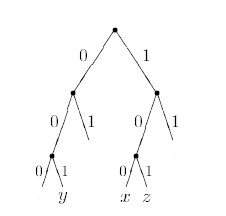
\includegraphics[scale=0.5]{img/int-trie.ps}
        \caption{An little-endian integer binary trie for the map 
          \{$ 1 \rightarrow a, 4 \rightarrow b, 5 \rightarrow c, 9 \rightarrow d$\}.} 
        \label{fig:int-trie}
       \end{center}
\end{figure}

\subsubsection*{Insertion of integer trie in Python}
Imperative implementation of insertion in Python can be easily given by translating
the pseudocode of the algorithm.

\lstset{language=Python}
\begin{lstlisting}
def trie_insert(t, key, value = None):
    if t is None:
        t = IntTrie()

    p = t
    while key != 0:
        if key & 1 == 0:
            if p.left is None:
                p.left = IntTrie()
            p = p.left
        else:
            if p.right is None:
                p.right = IntTrie()
            p = p.right
        key = key>>1
    p.value = value
    return t
\end{lstlisting}

In order to test this insertion program, some test helpers are provided:

\begin{lstlisting}
def trie_to_str(t, prefix=0, depth=0):
    to_str = lambda x: "%s" %x
    str="("+to_str(prefix)
    if t.value is not None:
        str += ":"+t.value
    if t.left is not None:
        str += ", "+trie_to_str(t.left, prefix, depth+1)
    if t.right is not None:
        str += ", "+trie_to_str(t.right, (1<<depth)+prefix, depth+1)
    str+=")"
    return str

def list_to_trie(l):
    t = None
    for x in l:
        t = trie_insert(t, x)
    return t

def map_to_trie(m):
    t = None
    for k, v in m.items():
        t = trie_insert(t, k, v)
    return t
\end{lstlisting}

Function trie\_to\_str can print the contents of trie in pre-order,
It doesn't only print the value of the ndoe, but also print the edge information.

Function list\_to\_trie can repeatly insert a list of keys into a trie, since the
default argument of value is None, so all data relative to keys are empty. If the
data isn't empty, function map\_to\_trie can insert a list of key-value pairs into 
the trie.

Then a test classe is given to encapasulate test cases:

\begin{lstlisting}
class IntTrieTest:
    def run(self):
        self.test_insert()

    def test_insert(self):
        t = None
        t = trie_insert(t, 0);
        t = trie_insert(t, 1);
        t = trie_insert(t, 4);
        t = trie_insert(t, 5);
        print trie_to_str(t)
        t1 = list_to_trie([1, 4, 5])
        print trie_to_str(t1)
        t2 = map_to_trie({4:'b', 1:'a', 5:'c', 9:'d'})
        print trie_to_str(t2)

if __name__ == "__main__":
    IntTrieTest().run()
\end{lstlisting}

Running this program will print the following result.

\begin{verbatim}
(0, (0, (0, (4))), (1, (1, (5))))
(0, (0, (0, (4))), (1, (1, (5))))
(0, (0, (0, (4:b))), (1:a, (1, (1, (9:d)), (5:c))))
\end{verbatim}

Please note that by pre-ordre traverse trie, we can get a 'lexical' order
result of the keys. For instance, the last result print the little-endian
format of key 1, 4, 5, 9 as below.

\begin{verbatim}
001
1
1001
101
\end{verbatim}

They are in lexcical order. We'll go back to this feature of trie later in 
alphabetic trie section.

% ================================================================
%               Look up in integer binary trie
% ================================================================
\subsection{Look up in integer binary trie} 

To look up a key in a little-endian integer binary trie. We take each
bit of the key from left (LSB), and go left or right according to if
the bit is 0, untill we consumes all bits. this algorithm can be described
as below pseudocode.

\begin{algorithmic}
\STATE $INT-TRIE-LOOKUP(T, x)$
  \WHILE{$x \neq 0$ and $T \neq NIL$}
    \IF{$EVEN(x) = TRUE$}
      \STATE $T \leftarrow LEFT(T)$
    \ELSE
      \STATE $T \leftarrow RIGHT(T)$
    \ENDIF
    \STATE $x \leftarrow x/2$
  \ENDWHILE
  \IF{$T \neq NIL$} \RETURN $DATA(T)$
  \ELSE \RETURN $NIL$ \ENDIF
\end{algorithmic}

\subsubsection*{Look up implemented in Haskell}
The algorithm in pseudocode is in imperative way, It can also be implemented 
recursivly like below Haskell program

\lstset{language=Haskell}
\begin{lstlisting}
search :: IntTrie a -> Key -> Maybe a
search Empty k = Nothing
search t 0 = value t
search t k = if even k then search (left t) (k `div` 2)
             else search (right t) (k `div` 2)
\end{lstlisting}

If trie is empty, we simply returns nothing; if key is zero we return the 
value of current node; in other case we recursively search either left
child or right child according to the LSB is 0 or not.

To test this program, we can write a smoke test case as following.

\begin{lstlisting}
testIntTrie = "t=" ++ (toString t) ++ 
              "\nsearch t 4: " ++ (show $ search t 4) ++
              "\nsearch t 0: " ++ (show $ search t 0)
    where
      t = fromList [(1, 'a'), (4, 'b'), (5, 'c'), (9, 'd')]

main = do
  putStrLn testIntTrie
\end{lstlisting}

This program will output these result.

\begin{verbatim}
t=(((. 0 (. 4:'b' .)) 0 .) 0 (((. 1 (. 9:'d' .)) 1 (. 5:'c' .)) 1:'a' .))
search t 4: Just 'b'
search t 0: Nothing
\end{verbatim}

\subsubsection*{Look up implemented in Python}
By translate the algorithm in pseudocode, we can easily get a python 
implementation.

\lstset{language=Python}
\begin{lstlisting}
def lookup(t, key):
    while key != 0 and (t is not None):
        if key & 1 == 0:
            t = t.left
        else:
            t = t.right
        key = key>>1
    if t is not None:
        return t.value
    else:
        return None
\end{lstlisting}

In this implementation, instead of using even-odd property, bit-wise
manipulation is used to test if a bit is 0 or 1.

Here is the smoke test of the lookup function.

\begin{lstlisting}
class IntTrieTest:
    #...
    def test_lookup(self):
        t = map_to_trie({4:'y', 1:'x', 5:'z'})
        print "look up 4: ", lookup(t, 4)
        print "look up 5: ", lookup(t, 5)
        print "look up 0: ", lookup(t, 0)
\end{lstlisting}

The output of the test cases is as below.

\begin{verbatim}
look up 4:  y
look up 5:  z
look up 0:  None
\end{verbatim}

% ================================================================
%               Int Patricia
% ================================================================
\section{Integer Patricia Tree} 
\label{int-patricia}

It's very easy to find the drawbacks of integer binary trie. Trie wasts a lot of 
spaces. Note in figure \ref{int-trie}, all nodes except leafs store the real data.
Typically, an integer binary trie contains many nodes only have one child.
It is very easy to come to the idea for improvement, to compress the chained nodes
which have only one child. Patricia is such a data structure invented by 
Donald R. Morrison in 1968. Patricia means practical algorithm to retrieve information coded
in aphanumeric\cite{patricia-morrison}. Wikipedia redirect Patricia as Radix tree.

Chris Okasaki gave his implementation of Integer Patricia tree in paper \cite{okasaki-int-map}. 
If we merge the chained nodes which have only one child together in figure \ref{fig:int-trie},
We can get a patricia as shown in figure \ref{fig:little-endian-patricia}.

\begin{figure}[htbp]
       \begin{center}
	\includegraphics[scale=0.5]{img/little-endian-patricia.ps}
        \caption{Little endian patricia for the map 
                        \{$ 1 \rightarrow a, 4 \rightarrow b, 5 \rightarrow c, 9 \rightarrow d$\}.} 
        \label{fig:little-endian-patricia}
       \end{center}
\end{figure}

From this figure, we can found that they keys of sibling nodes have the longest common prefix.
They only branches out at certain bit. It means that we can save a lot of data by storing the common
prefix. 

Different from integer Trie, using big-endian integer in Patricia doesn't cause the problem mentioned
in section \ref{int-trie}. Becasue all zero bits before MSB can be just omitted to save space. Big-endian
interger is more natural than little-endian integer. Chris Okasaki list some significant advantages
of big-endian Patricia trees \cite{okasaki-int-map}.

% ================================================================
%                 Definition of int patricia tree
% ================================================================
\subsection{Definition of Integer Patricia tree}
Integer Patricia tree is a speical kind of binary tree, it is
\begin{itemize}
\item either a leaf node contains an integer key and a value
\item or a branch node, contains a left child and a right child. The
integer keys of two children shares the longest common prefix bits,
the next bit of the left child's key is zero while it is one for right
child's key.
\end{itemize}

\subsubsection*{Definition of big-endian integer Patricia tree in Haskell}
If we translate the above recurisive definition to Haskell, we can get
below Integer Patrica Tree code.

\lstset{language=Haskell}
\begin{lstlisting}
data IntTree a = Empty 
               | Leaf Key a
               | Branch Prefix Mask (IntTree a) (IntTree a) -- prefix, mask, left, right

type Key = Int
type Prefix = Int
type Mask = Int
\end{lstlisting}

In order to tell from which bit the left and right children differ, a
mask is recorded by the branch node. Typically, a mask is $2^n$, all
lower bits than n doesn't belong to common prefix

\subsubsection*{Definition of big-endian integer Patricia tree in Python}
Such definition can be represent in Python similarly. Some helper
functions are provided for easy operation later on.

\lstset{language=Python}
\begin{lstlisting}
class IntTree:
    def __init__(self, key = None, value = None):
        self.key = key
        self.value = value
        self.prefix = self.mask = None
        self.left = self.right = None

    def set_children(self, l, r):
        self.left = l
        self.right = r

    def replace_child(self, x, y):
        if self.left == x:
            self.left = y
        else:
            self.right = y

    def is_leaf(self):
        return self.left is None and self.right is None

    def get_prefix(self):
        if self.prefix is None:
            return self.key
        else:
            return self.prefix
\end{lstlisting}

% ================================================================
%                 Insertion of int patricia tree
% ================================================================
\subsection{Insertion of Integer Patricia tree}
When insert a key into a integer Patricia tree, if the tree is empty,
we can just create a leaf node with the given key and data. (as shown
in figure \ref{fig:int-patricia-insert-a}).

\begin{figure}[htbp]
       \begin{center}
	\includegraphics[scale=1]{img/int-patricia-insert-a.ps}
        \caption{(a). Insert key 12 to an empty patricia tree.}
        \label{fig:int-patricia-insert-a}
       \end{center}
\end{figure}

If the tree only contains a leaf node x, we can create a branch, put the new
key and data as a leaf y of the branch. To determin if the new leaf y
should be left node or right node. We need find the longest common prefix
of x and y, for example if key(x) is 12 (1100 in binary), key(y) is 15
(1111 in binary), then the longest common prefix is $11oo$. The $o$
denotes the bits we don't care about. we can use an integer to mask
the those bits. In this case, the mask number is 4 (100 in binary).
The next bit after the prefix presents $2^1$. It's 0 in key(x), while
it is 1 in key(y). So we put x as left child and y as right
child. Figure \ref{fig:int-patricia-insert-b} shows this case.

\begin{figure}[htbp]
       \begin{center}
	\includegraphics[scale=1]{img/int-patricia-insert-b.ps}
        \caption{(b). Insert key 15 to the result tree in (a).}
        \label{fig:int-patricia-insert-b}
       \end{center}
\end{figure}

If the tree is neither empty, nor a leaf node, we need firstly check
if the key to be inserted matches common prefix with root node. If it
does, then we can recursively insert the key to the left child or right child
according to the next bit. For instance, if we want to
insert key 14 (1110 in binary) to the result tree in figure 
\ref{fig:int-patricia-insert-b}, since it has common prefix $11oo$,
and the next bit (the bit of $2^1$) is 1, so we tried to insert 14 to
the right child. Otherwise, if the key to be inserted desn't match the
common prefix with the root node, we need branch a new leaf
node. Figure \ref{fig:int-patricia-insert-c} shows these 2 different cases.

\begin{figure}[htbp]
       \begin{center}
	\includegraphics[scale=0.5]{img/int-patricia-insert-c.ps}
	\includegraphics[scale=0.5]{img/int-patricia-insert-d.ps}
        \caption{(c). Insert key 14 to the ressult tree in (b);
	(d). Insert key 5 to the result tree in (b).}
        \label{fig:int-patricia-insert-c}
       \end{center}
\end{figure}

Summarize the above cases, the insertion of integer patricia can be described
with the following algorithm.

\begin{algorithmic}
\STATE $INT-PATRICIA-INSERT(T, x, data)$
\IF{$T = NIL$}
   \STATE $T \leftarrow CREATE-LEAF(x, data)$
   \RETURN $T$
\ENDIF

\STATE $y \leftarrow T$
\STATE $p \leftarrow NIL$
\WHILE{$LEAF(y) = TRUE$ and $MATCH(x, PREFIX(y), MASK(y))$}
  \STATE $p \leftarrow y$
  \IF{$ZERO(x, MASK(y)) = TRUE$}
    \STATE $y \leftarrow LEFT(y)$
  \ELSE
    \STATE $y \leftarrow RIGHT(y)$
  \ENDIF
\ENDWHILE

\IF{$LEAF(y) = TRUE$ and $x = KEY(y)$}
  \STATE $DATA(y) \leftarrow data$ 
\ELSE
  \STATE $z \leftarrow BRANCH(y, CREATE-LEAF(x, data))$
  \IF{$p = NIL$}
    \STATE $T \leftarrow z$
  \ELSE
    \IF{$LEFT(p) = y$}
      \STATE $LEFT(p) \leftarrow z$
    \ELSE
      \STATE $RIGHT(p) \leftarrow z$
    \ENDIF
  \ENDIF
\ENDIF
\RETURN $T$
\end{algorithmic}

In the above algorithm, MATCH procedure test if an integer key $x$, has 
the same prefix of node y above the mask bit. For instance,
Suppose the prefix of node y can be denoted as 
$p(n), p(n-1), ..., p(i), ..., p(0)$ in binary, key x is
$k(n), k(n-1), ..., k(i), ..., k(0)$, and mask of node y is 
$100...0=2^i$, if and only if $p(j)=k(j)$ for all $i \leq j \leq n$, 
we say the key matches.

\subsubsection*{Insertion of big-endian integer Patricia tree in Haskell}
Insertion of big-endian integer Patricia tree can be implemented in Haskell
by Change the above algorithm to recursive approach.

\lstset{language=Haskell}
\begin{lstlisting}
-- usage: insert tree key x
insert :: IntTree a -> Key -> a -> IntTree a
insert t k x 
   = case t of
       Empty -> Leaf k x
       Leaf k' x' -> if k==k' then Leaf k x
                     else join k (Leaf k x) k' t -- t@(Leaf k' x')
       Branch p m l r
          | match k p m -> if zero k m
                           then Branch p m (insert l k x) r
                           else Branch p m l (insert r k x)
          | otherwise -> join k (Leaf k x) p t -- t@(Branch p m l r)
\end{lstlisting}

The match, zero and join functions in this program are defined as below.
\begin{lstlisting}
-- join 2 nodes together.
-- (prefix1, tree1) ++ (prefix2, tree2)
--  1. find the longest common prefix == common(prefix1, prefix2)
--         prefix1 = a(n),a(n-1),...a(i+1),a(i),x...
--         prefix2 = a(n),a(n-1),...a(i+1),a(i),y...
--         prefix  = a(n),a(n-1),...a(i+1),a(i),00...0
--  2. mask bit = 100...0b (=2^i)
--         so mask is something like, 1,2,4,...,128,256,...
--  3. if      x=='0', y=='1' then (tree1=>left, tree2=>right), 
--     else if x=='1', y=='0' then (tree2=>left, tree1=>right).
join :: Prefix -> IntTree a -> Prefix -> IntTree a -> IntTree a
join p1 t1 p2 t2 = if zero p1 m then Branch p m t1 t2
                                else Branch p m t2 t1 
    where
      (p, m) = lcp p1 p2

-- 'lcp' means 'longest common prefix'
lcp :: Prefix -> Prefix -> (Prefix, Mask)
lcp p1 p2 = (p, m) where
    m = bit (highestBit (p1 `xor` p2))
    p = mask p1 m

-- get the order of highest bit of 1.
-- For a number x = 00...0,1,a(i-1)...a(1)
-- the result is i
highestBit :: Int -> Int
highestBit x = if x==0 then 0 else 1+highestBit (shiftR x 1)

-- For a number x = a(n),a(n-1)...a(i),a(i-1),...,a(0)
-- and a mask m = 100..0 (=2^i)
-- the result is a(n),a(n-1)...a(i),00..0
mask :: Int -> Mask -> Int
mask x m = (x .&. complement (m-1)) -- complement means bitwise not.


-- Test if the next bit after mask bit is zero
-- For a number x = a(n),a(n-1)...a(i),1,...a(0)
-- and a mask   m = 100..0 (=2^i)
-- because the bit next to a(i) is 1, so the result is False
-- For a number y = a(n),a(n-1)...a(i),0,...a(0) the result is True.
zero :: Int -> Mask -> Bool
zero x m = x .&. (shiftR m 1) == 0

-- Test if a key matches a prefix above of the mask bit
-- For a prefix: p(n),p(n-1)...p(i)...p(0)
--     a key:    k(n),k(n-1)...k(i)...k(0)
-- and a mask:                 100..0 = (2^i)
-- If and only if p(j)==k(j), i<=j<=n the result is True
match :: Key -> Prefix -> Mask -> Bool
match k p m = (mask k m) == p
\end{lstlisting}

In order to test the above insertion program, some test helper functions
are provided.

\begin{lstlisting}
-- Generate a Int Patricia tree from a list
-- Usage: fromList [(k1, x1), (k2, x2),..., (kn, xn)]
fromList :: [(Key, a)] -> IntTree a
fromList xs = foldl ins Empty xs where
    ins t (k, v) = insert t k v

toString :: (Show a)=>IntTree a -> String
toString t =
    case t of
      Empty -> "."
      Leaf k x -> (show k) ++ ":" ++ (show x)
      Branch p m l r -> "[" ++ (show p) ++ "@" ++ (show m) ++ "]" ++ 
                        "(" ++ (toString l) ++ ", " ++ (toString r) ++ ")"

\end{lstlisting}

With these helpers, insertion can be test as the following.

\begin{lstlisting}
testIntTree = "t=" ++ (toString t) 
    where
      t = fromList [(1, 'x'), (4, 'y'), (5, 'z')]

main = do
  putStrLn testIntTree
\end{lstlisting}

This test will output:

\begin{verbatim}
t=[0@8](1:'x', [4@2](4:'y', 5:'z'))
\end{verbatim}

This is a Patrica like 

\subsubsection*{Insertion of big-endian integer Patricia tree in Python}
in python
\lstset{language=Python}
\begin{lstlisting}
...
\end{lstlisting}

% ================================================================
%                 Lookup in int patricia tree
% ================================================================
\subsection{Look up in Integer Patricia tree}
look up integer patricia tree...

pseudocode...

\subsubsection*{Look up in big-endian integer Patricia tree in Haskell}
in Haskell...

\subsubsection*{Look up in big-endian integer Patricia tree in Python}
in Python...
\lstset{language=Python}
\begin{lstlisting}
...
\end{lstlisting}

% ================================================================
%                 Alphabetic trie
% ================================================================
\section{Alphabetic Trie}
Alphabetic trie...

% ================================================================
%                 Definition of Alphabetic trie
% ================================================================
\subsection{Definition of alphabetic Trie}
Definition...

\subsubsection*{Definition of alphabetic Trie in Haskell}
in Haskell...

\lstset{language=Haskell}
\begin{lstlisting}
...
\end{lstlisting}

\subsubsection*{Definition of alphabetic Trie in Python}
in Python...

\lstset{language=Python}
\begin{lstlisting}
...
\end{lstlisting}

% ================================================================
%                 Insertion of Alphabetic trie
% ================================================================
\subsection{Insertion of aplhabetic trie}
Insertion...

Pseudocode...

\subsubsection*{Insertion of alphabetic trie in Haskell}
in haskell...

\lstset{language=Haskell}
\begin{lstlisting}
...
\end{lstlisting}

\subsubsection*{Insertion of alphabetic trie in C++}
in C++...

\lstset{language=C++}
\begin{lstlisting}
...
\end{lstlisting}


\subsubsection*{Insertion of alphabetic trie in Python}
in python...

\lstset{language=Python}
\begin{lstlisting}
...
\end{lstlisting}

\subsubsection*{Insertion of alphabetic trie in Scheme/Lisp}
in scheme/lisp...

\lstset{language=lisp}
\begin{lstlisting}
...
\end{lstlisting}

% ================================================================
%                 Look up in Alphabetic trie
% ================================================================
\subsection{Look up in aplhabetic trie}
Insertion...

Pseudocode...

\subsubsection*{Look up in alphabetic trie in Haskell}
in haskell...

\lstset{language=Haskell}
\begin{lstlisting}
...
\end{lstlisting}

\subsubsection*{Look up in alphabetic trie in C++}
in C++...

\lstset{language=C++}
\begin{lstlisting}
...
\end{lstlisting}


\subsubsection*{Look up in alphabetic trie in Python}
in python...

\lstset{language=Python}
\begin{lstlisting}
...
\end{lstlisting}

\subsubsection*{Look up in alphabetic trie in Scheme/Lisp}
in scheme/lisp...

\lstset{language=lisp}
\begin{lstlisting}
...
\end{lstlisting}

% ================================================================
%                 Alphabetic Patricia Tree
% ================================================================
\section{Alphabetic Patricia Tree}
Alphabetic patricia...

% ================================================================
%                 Definition of Alphabetic Patricia Tree
% ================================================================
\subsection{Definition of alphabetic Patricia Tree}
Definition...

\subsubsection*{Definition of alphabetic Patricia Tree in Haskell}
in Haskell...

\lstset{language=Haskell}
\begin{lstlisting}
...
\end{lstlisting}

\subsubsection*{Definition of alphabetic Patricia Tree in Python}
in Python...

\lstset{language=Python}
\begin{lstlisting}
...
\end{lstlisting}

% ================================================================
%                 Insertion of Alphabetic Patrica Tree
% ================================================================
\subsection{Insertion of aplhabetic Patricia Tree}
Insertion...

Pseudocode...

\subsubsection*{Insertion of alphabetic Patrica Tree in Haskell}
in haskell...

\lstset{language=Haskell}
\begin{lstlisting}
...
\end{lstlisting}

\subsubsection*{Insertion of alphabetic Patricia in C++}
in C++...

\lstset{language=C++}
\begin{lstlisting}
...
\end{lstlisting}


\subsubsection*{Insertion of alphabetic Patrica Tree in Python}
in python...

\lstset{language=Python}
\begin{lstlisting}
...
\end{lstlisting}

\subsubsection*{Insertion of alphabetic Patrica Tree in Scheme/Lisp}
in scheme/lisp...

\lstset{language=lisp}
\begin{lstlisting}
...
\end{lstlisting}

% ================================================================
%                 Look up in Alphabetic Patrica Tree
% ================================================================
\subsection{Look up in aplhabetic Patricia Tree}
Insertion...

Pseudocode...

\subsubsection*{Look up in alphabetic Patrica Tree in Haskell}
in haskell...

\lstset{language=Haskell}
\begin{lstlisting}
...
\end{lstlisting}

\subsubsection*{Look up in alphabetic Patrica Tree in C++}
in C++...

\lstset{language=C++}
\begin{lstlisting}
...
\end{lstlisting}


\subsubsection*{Look up in alphabetic Patricia Tree in Python}
in python...

\lstset{language=Python}
\begin{lstlisting}
...
\end{lstlisting}

\subsubsection*{Look up in alphabetic Patricia Tree in Scheme/Lisp}
in scheme/lisp...

\lstset{language=lisp}
\begin{lstlisting}
...
\end{lstlisting}

% ================================================================
%                 Trie and Patrica used in Industry
% ================================================================
\section{Trie and Patricia used in Industry}
...

% ================================================================
%                 Suffix Trie
% ================================================================
\section{Suffix Trie}
...

\subsection{construction of suffix trie}
...

\section{Suffix Tree}
...

\subsection{construction algorithms of suffix tree}

\section{Suffix tree used in Industry}

% ================================================================
%                 Appendix
% ================================================================
\section{Appendix} \label{appendix}
%\appendix
All programs provided along with this article. They are free for downloading.
\begin{itemize}
\item IntTrie.hs, Haskell version of little-endian integer Trie, with test cases. I compiled
and tested it with GHC 6.10.4.
\item inttrie.cpp,
\item inttrie.py, Python version of little-endian integer Trie, with test cases. Tested
with Python 2.5.1
\item inttrie.scm,
\item IntPatricia.hs,
\item intpatricia.cpp,
\item intpatricia.py,
\item intpatricia.scm
\item Trie.hs,
\item trie.cpp,
\item trie.py,
\item trie.scm,
\item Patricia.hs,
\item patricia.cpp,
\item patricia.py,
\item patricia.scm,
\item xxx.scm, Scheme version of xxxx and test cases. Tested
with MIT/Scheme 14.9
\end{itemize}

Besides them, I use graphviz to draw most of the figures in this post. In order to
translate the Trie, Patrica and Suffix Tree output to dot language scripts. I wrote a python program.
it can be used like this.

\begin{verbatim}
trie2dot.py -o foo.dot -t patricia "1:x, 4:y, 5:z"
trie2dot.py -o foo.dot -t trie "001:one, 101:five, 100:four"
\end{verbatim}

This helper scripts can also be downloaded with this article.

download position: http://sites.google.com/site/algoxy/trie/trie.zip

\begin{thebibliography}{99}

\bibitem{CLRS}
Thomas H. Cormen, Charles E. Leiserson, Ronald L. Rivest and Clifford Stein. 
``Introduction to Algorithms, Second Edition''. ISBN:0262032937. The MIT Press. 2001

\bibitem{okasaki-int-map}
Chris Okasaki and Andrew Gill. ``Fast Mergeable Integer
Maps''. Workshop on ML, September 1998, pages 77-86, http://www.cse.ogi.edu/~andy/pub/finite.htm

\bibitem{patricia-morrison}
D.R. Morrison, ``PATRICIA -- Practical Algorithm To Retrieve  Information Coded In Alphanumeric", Journal of the ACM, 15(4), October 1968, pages 514-534.

\bibitem{wiki-suffix-tree}
Suffix Tree, Wikipedia. http://en.wikipedia.org/wiki/Suffix\_tree

\bibitem{wiki-trie}
Trie, Wikipedia. http://en.wikipedia.org/wiki/Trie

\end{thebibliography}

\ifx\wholebook\relax\else
\end{document}
\fi
